\documentclass[12pt,a4paper]{article}

\usepackage{amsmath}
\usepackage{graphics,graphicx}
\usepackage{txfonts}
\usepackage{natbib}
\usepackage{xcolor}
\usepackage{xspace}
\usepackage{hyperref}
\usepackage{etoolbox}
\usepackage{lastpage}
\usepackage{sidecap}
% \usepackage[cm]{fullpage}
\usepackage[a4paper,headsep=5pt,footskip=23pt]{geometry}

\makeatletter

% Patch case where name and year are separated by aysep
\patchcmd{\NAT@citex}
  {\@citea\NAT@hyper@{%
     \NAT@nmfmt{\NAT@nm}%
     \hyper@natlinkbreak{\NAT@aysep\NAT@spacechar}{\@citeb\@extra@b@citeb}%
     \NAT@date}}
  {\@citea\NAT@nmfmt{\NAT@nm}%
   \NAT@aysep\NAT@spacechar\NAT@hyper@{\NAT@date}}{}{}

% Patch case where name and year are separated by opening bracket
\patchcmd{\NAT@citex}
  {\@citea\NAT@hyper@{%
     \NAT@nmfmt{\NAT@nm}%
     \hyper@natlinkbreak{\NAT@spacechar\NAT@@open\if*#1*\else#1\NAT@spacechar\fi}%
       {\@citeb\@extra@b@citeb}%
     \NAT@date}}
  {\@citea\NAT@nmfmt{\NAT@nm}%
   \NAT@spacechar\NAT@@open\if*#1*\else#1\NAT@spacechar\fi\NAT@hyper@{\NAT@date}}
  {}{}

\makeatother



\newcommand{\anote}[2]{{\color{cyan}#1}: {\color{blue} #2}}
\newcommand{\rephrase}[1]{{\color{pink}Reformulate}: {\color{red}\it #1}}
\newcommand{\cneeded}{{\color{red}(citation needed)}\xspace}
\newcommand{\todo}[1]{{\color{teal}TODO: #1}\xspace}
\newcommand{\tabnote}[1]{$^{\rm #1}$\xspace}
\newcommand{\tabnotep}[1]{\tabnote{(#1)}\xspace}
\newcommand{\hlink}[1]{\url{http://#1}\xspace}
\newcommand{\changed}[1]{#1}

\newcommand{\rfig}[1]{Fig.~\ref{#1}}
\newcommand{\rfigs}[1]{Figs.~\ref{#1}}
\newcommand{\req}[1]{Eq.~\ref{#1}}
\newcommand{\reqs}[1]{Eqs.~\ref{#1}}
\newcommand{\rtab}[1]{Table \ref{#1}}
\newcommand{\rtabs}[1]{Tables \ref{#1}}
\newcommand{\rapp}[1]{Appendix \ref{#1}}
\newcommand{\rapps}[1]{Appendices \ref{#1}}
\newcommand{\rsec}[1]{subsection \ref{#1}}
\newcommand{\rsecs}[1]{sections \ref{#1}}
\newcommand{\rfnote}[1]{footnote \ref{#1}}
\newcommand{\rfnotes}[1]{footnotes \ref{#1}}

\newcommand{\via}{{\it via}\xspace}

\newcommand{\herschel}{{\it Herschel}\xspace}
\newcommand{\spitzer}{{\it Spitzer}\xspace}
\newcommand{\hubble}{{\it Hubble}\xspace}
\newcommand{\hst}{{\it HST}\xspace}
\newcommand{\jwst}{{\it JWST}\xspace}
\newcommand{\subaru}{{\it Subaru}\xspace}
\newcommand{\GALEX}{{\it GALEX}\xspace}

\newcommand{\um}{\mu{\rm m}}
\newcommand{\uJy}{\mu{\rm Jy}}
\newcommand{\mJy}{{\rm mJy}}
\newcommand{\mad}{{\rm MAD}}
\newcommand{\nmad}{{\rm NMAD}}
\newcommand{\median}[1]{\left<#1\right>}
\newcommand{\mean}[1]{\left<#1\right>}
\newcommand{\logd}{\log_{10}}
\newcommand{\sfr}{{\rm SFR}}
\newcommand{\sfruv}{{\rm SFR}_{\rm UV}}
\newcommand{\sfrir}{{\rm SFR}_{\rm IR}}
\newcommand{\sfrms}{{\rm SFR}_{\rm MS}}
\newcommand{\ssfr}{{\rm sSFR}}
\newcommand{\lir}{L_{\rm IR}}
\newcommand{\lfir}{L_{\rm FIR}}
\newcommand{\irx}{\rm IRX}
\newcommand{\leight}{L_8}
\newcommand{\ireight}{{\rm IR8}}
\newcommand{\cplus}{[\ion{C}{II}]}
\newcommand{\luv}{L_{\rm UV}}
\newcommand{\lsun}{L_\odot}
\newcommand{\msun}{{\rm M}_\odot}
\newcommand{\mdense}{{\rm M}_{\rm dense}}
\newcommand{\mgas}{{\rm M}_{\rm gas}}
\newcommand{\mhalo}{{\rm M}_{\rm halo}}
\newcommand{\fgas}{f_{\rm gas}}
\newcommand{\Mpc}{{\rm Mpc}}
\newcommand{\Gyr}{{\rm Gyr}}
\newcommand{\Myr}{{\rm Myr}}
\newcommand{\yr}{{\rm yr}}
\newcommand{\dex}{{\rm dex}}
\newcommand{\mstar}{M_\ast}
\newcommand{\snr}{{\rm SNR}}
\newcommand{\snu}{S_{\!\nu}}
\newcommand{\tdust}{T_{\rm dust}}
\newcommand{\rhosfr}{\rho_{\sfr}}
\newcommand{\rhostar}{\rho_{\ast}}
\newcommand{\rsb}{R_{\rm SB}}
\newcommand{\uvj}{$UVJ$\xspace}
\newcommand{\bzk}{$BzK$\xspace}
\newcommand{\bt}{B/T}
\newcommand{\rdisk}{R_{\rm disk}}
\newcommand{\rbulge}{R_{\rm bulge}}
\newcommand{\sersic}{S\'ersic\xspace}

\newcommand{\halpha}{${\rm H}_\alpha$\xspace}
\newcommand{\Ks}{$K_{\rm s}$\xspace}
\newcommand{\celib}{CE01\xspace}
\newcommand{\sextractor}{{\sc SExtractor}\xspace}
\newcommand{\galfit}{{\sc Galfit}\xspace}

\newcommand\efp{%
  \newgeometry{left=1.8cm,bottom=2.0cm,right=1.8cm,top=1.8cm} %
  \resetHeadWidth %
  \renewcommand{\headrulewidth}{0.4pt} %
  \noindent %
}

\makeatletter
\newcommand{\resetHeadWidth}{\fancy@setoffs}
\makeatother

% Alter some LaTeX defaults for better treatment of figures:
% See p.105 of "TeX Unbound" for suggested values.
% See pp. 199-200 of Lamport's "LaTeX" book for details.
%   General parameters, for ALL pages:
\renewcommand{\topfraction}{0.95}  % max fraction of floats at top
\renewcommand{\bottomfraction}{0.8} % max fraction of floats at bottom
%   Parameters for TEXT pages (not float pages):
\setcounter{topnumber}{2}
\setcounter{bottomnumber}{2}
\setcounter{totalnumber}{4}     % 2 may work better
\setcounter{dbltopnumber}{2}    % for 2-column pages
\renewcommand{\dbltopfraction}{0.9} % fit big float above 2-col. text
\renewcommand{\textfraction}{0.07}  % allow minimal text w. figs
%   Parameters for FLOAT pages (not text pages):
\renewcommand{\floatpagefraction}{0.9}  % require fuller float pages
% N.B.: floatpagefraction MUST be less than topfraction !!
\renewcommand{\dblfloatpagefraction}{0.9} % require fuller float pages

\begin{document}
\newgeometry{left=1.8cm,bottom=2.0cm,right=1.8cm,top=1.8cm}

\section{Creating the mock catalog}

The main idea behind the generation process of this mock catalog is that everything can be statistically inferred from the redshift, the stellar mass and the ``star-forming'' flag of each galaxy. The procedure is therefore composed of two main steps: first, generate a realistic distribution of masses at different redshifts both for active and passive galaxies using observed mass-functions; second, estimate all the other physical properties using statistical recipes: morphology, $\sfr$, attenuation, optical colors, and sky-projected position. I now describe each calculation in detail.


\subsection{Generating redshifts and masses}

The purpose of the mock catalog is the simulate a field similar to the GOODS--South CANDELS field. Therefore, in order to most closely mimic the properties of this field, I have estimate conditional mass functions at different redshifts, as described in my paper (Schreiber et al.~2014). Briefly, the whole GOODS--South catalog is cut at $H<26$ to ensure high completeness, split in two population of ``active'' and ``passive'' galaxies according to the UVJ color-color selection, and further split in multiple redshift bins from $z=0.3$ to $z=4.5$. I have used the masses and redshifts computed by Maurilio Pannella using the CANDELS photometry, but I can easily switch to the official CANDELS mass and redshift catalog if needed. Then, I simply computed the mass distribution of each of these sub-samples, performing 1st order completeness corrections, and fit a double Schechter law. Using these fits, I can generate mass functions down to arbitrarily low stellar masses. To reach higher redshifts, I have used the mass functions calculated by Grazian et al.~(2014) for $z < 7.5$. The $z=0$ mass functions is adapted from Baldry et al.~(2012) (converted from Chabrier to Salpeter), but it should not matter much since we are aiming for pencil-beam surveys which contain very few local galaxies.

Once this is done, I define a fine grid of redshifts, say from $z=0.01$ to $z=6$ with $\Delta z \simeq 0.1 \times (1 + z)$ (imposing a minimum $\Delta z > 0.1$), and I choose the sky area of the mock catalog (here I took an area similar to the catalog you first produced with Stuff, i.e.~ $17 \times 17\,{\rm arcmin}$). In each redshift bin, I interpolate the above mass-functions to a redshift equal to the center of the current bin, multiply it by the volume of Universe probed by the survey in this bin, and generate masses following the distributions of both passive and active galaxies (the two populations are identified by a flag in the catalog), from $\mstar = M_{\rm min}$ to $\mstar = M_{\rm max}$. I chose $M_{\rm max} = 10^{12}\,\msun$, and $M_{\rm min}$ can be chosen either to be constant (e.g.~$10^{7}\,\msun$) or to vary with redshift so as to reach a given magnitude limit in the selection band (so you can chose to generate a catalog which is complete down to $H < 27$, for example). This later step uses the library optical SEDs described below to estimate roughly the mass completeness.

Now, the mock catalog has exactly the same mass and redshift distribution as the CANDELS catalog in GOODS--South. This is nice, but one has to keep in mind that, by construction, this also means that we have imposed the same cosmic variance than in GOODS--South.


\subsection{Generating morphology}

The Stuff program was not only generating photometry, but also detailed morphology and bulge-to-disk decomposition in each band. In order to be able to plug this new mock catalog in Skymaker directly, I also generate these informations.

The first important quantity is the bulge-to-total ratio $B/T$, which tells how much of the \emph{mass} of the galaxy goes into the bulge, as opposed to the disk. I generate this quantity using the relations between $B/T$ and $\mstar$ published by Lang et al.~(2014). These relations are conveniently provided both for active and passive galaxies, at different redshifts. They report no strong redshift evolution between $z=1$ and $z=2$, so I chose to make the $B/T$ simply depend on mass following
\begin{align}
(B/T)_{\rm active} &= 0.2 \times \left(\frac{\mstar}{10^{10}}\right)^{0.27} \times 10^{G(0.2)}\,\text{and} \\
(B/T)_{\rm passive} &= 0.5 \times \left(\frac{\mstar}{10^{10}}\right)^{0.1} \times 10^{G(0.2)}\,,
\end{align}
where $G(\sigma)$ is a zero-mean Gaussian noise of amplitude $\sigma$. The $B/T$ is then clamped to $0 \leq B/T \leq 1$. This quantity will be used later to define the colors of the galaxies.

The other set of morphological properties we need to generate are the axis ratio, position angle and size of both the disk and the bulge component of each galaxy. I chose to give the same position angle to both components, which is chosen randomly with uniform probability between $-90\deg$ and $+90\deg$. The axis ratio is generated following the distribution observed in the real catalogs. For the disk (resp.~bulge), I took a sample of galaxies with S\'ersic index $n<1.5$ (resp.~$n>2.5$) and computed their axis ratio distribution. The result is shown in \rfig{FIG:axis_ratio}. I used these distributions to generate the axis ratios of both disks and bulges in the mock catalog.

\begin{SCfigure}
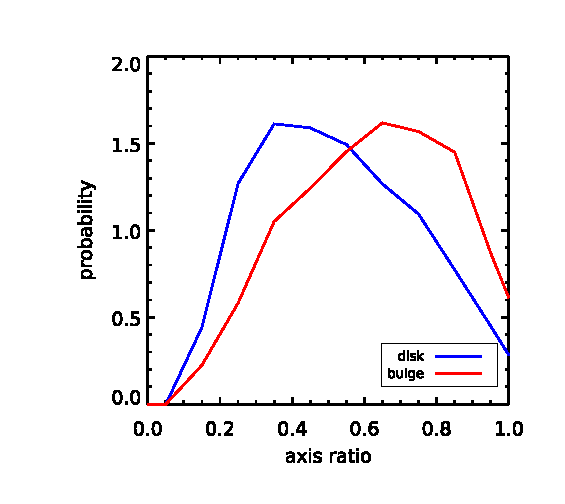
\includegraphics[width=0.5\textwidth]{axis_ratio}
\caption{\label{FIG:axis_ratio} Observed axis ratio distribution of disk-dominated ($n<1.5$) and bulge-dominated ($n>2.5$) galaxies. S\'ersic fits were taken from the CANDELS wiki, and were produced by Arjen van der Wel. Note that I also added a cut in stellar mass, in order not to be polluted by low mass faint galaxies ($\mstar > 10^{9}\,\msun$ for disks, $\mstar > 3\times10^{10}\,\msun$ for bulges).}
\end{SCfigure}

To estimate the sizes, I used the same sub-samples and looked at the relation between the observed $H$-band size, the mass, and the redshift. I ended up with the following relations
\begin{align}
R_{\rm disk} &= \begin{cases}
(1+z)^{-1.25} \times \left(\frac{\mstar}{10^{10}}\right)^{0.17} \times 10^{G(0.2)}\,&\text{for $z < 1.5$,} \\
0.4 \times (1+z)^{-0.25} \times \left(\frac{\mstar}{10^{10}}\right)^{0.17} \times 10^{G(0.2)}\,&\text{for $z > 1.5$, and}
\end{cases} \\
R_{\rm bulge} &= (1+z)^{-2.5} \times \left(\frac{\mstar}{10^{10}}\right)^{0.7} \times 10^{G(0.2)}\,,
\end{align}


\subsection{Generating star formation rate \label{SEC:sfr}}

This step is simple. I used the Main Sequence approach, which attributes a ``main sequence'' $\sfr$ to every galaxy, knowing its redshift and its stellar mass. I used the $\sfr_{\rm MS}$ published in my paper (Schreiber et al.~2014, Eq.~9). On top of this, a random lognormal scatter of $0.3\,\dex$ is added, so that
\begin{align}
\rsb &= 10^{G(0.3)} \\
\sfr &= \sfr_{\rm MS} \times \, \rsb.
\end{align}

This quantity, $\rsb$, the ``starburstiness'', will be used later to generate the IR photometry.

Then, I split this $\sfr$ between obscured and non-obscured components. The obscured component generates the IR fluxes, while the non-obscured component emerges naturally in the UV. To do so, I use the evolution of $\irx \equiv \lir/\luv$ I saw when doing stacking for my latest paper, which gives
\begin{align}
\irx &= \begin{cases}
15.8 \times \left(\frac{\mstar}{3 \times 10^{10}}\right)^{0.45\, z + 0.35}\,\
&\text{for $z<3$} \\
15.8 \times \left(\frac{\mstar}{3 \times 10^{10}}\right)^{1.7}\,&\text{for $z>3$.}
\end{cases}
\end{align}

From there is it then simple to recover $\lir$ and $\luv$, and therefore the obscured and non-obscured part of the $\sfr$. Note finally that passive galaxies are given zero $\sfr$.


\subsection{Generating optical colors}

To pick an optical SED for each galaxy, I choose to work with the \uvj color-color diagram. In there, passive galaxies occupy a well defined region (red cloud), while star-forming galaxies form a sort of ``sequence'', which is actually generated by the attenuation vector (assuming the Calzetti law, see e.g.~Williams et al. 2009, Fig.~8). This is useful, because it is known (e.g.~Pannella et al.~2014) that the attenuation correlates strongly with the stellar mass. I used this fact to associate colors to active and passive galaxies, again starting only from their redshift and masses. You can also take a look at Fig.~1 in my paper (Schreiber et al.~2014) to see the trends.

Passive galaxies are well condensed in a fixed region, close to $V-J = 1.25$ and $U-V = 1.85$, so they are simple to generate. There is a small trend with stellar mass as well. It is not very important, but I will simulate it for completeness. The principle is to put all passive galaxies at the position given just above, shift them according to the attenuation vector with a stellar mass trend, and add some Gaussian noise to the colors. The final colors are chosen following
\begin{align}
A &= 0.1 \times (\log_{10}(\mstar/\msun) - 11) + G(0.1)\,, \\
(V-J)_{\rm passive} &= 1.25 + A + G(0.1)\,, \\
(U-V)_{\rm passive} &= 1.85 + 0.88 \times A + G(0.1)\,.
\end{align}
Note that the ``shift'' $A$ is clamped to the range $[-0.1,0.2]$ so that galaxies do not leave the red cloud.

For star-forming galaxies, one needs to be a bit more subtle because their colors vary a lot more. As can be seen in Fig.~1 from Schreiber et al.~(2014), star-forming galaxies populate different regions of the \uvj diagram depending on the stellar mass and redshift: massive galaxies are preferentially located on the top-right corner (red $U-V$ and $V-J$ colors), while low-mass galaxies are at the bottom-left (blue in $U-V$ and $V-J$), and they are shifted to bluer colors at higher redshift. This can be due either to a difference of attenuation, or younger ages. In any case, we can parametrize this evolution.

To do so, I took a sample of \uvj star-forming galaxies in GOODS--South, and split it in mass bins. I further decompose each of these bins by slicing in redshift, and compute the median $U-V$ and $V-J$ colors. This gives me a set of tracks in the \uvj diagram, which are reproduced in \rfig{FIG:uvj_track} (left). It turns out that these tracks fall roughly on a fixed line of slope $0.65$. So I computed the projection of the tracks on that line, and parametrized its evolution as
\begin{align}
A_0 &= 0.58 \times {\rm erf}(\log_{10}(\mstar/\msun) - 10) + 1.39\,, \\
A_s &= \begin{cases}
-0.34 + 0.3 \times \log_{10}\left(\frac{\mstar}{2.2 \times 10^{10}\,\msun}\right)\,&\text{for $\mstar > 2.2 \times 10^{10}\,\msun$,} \\
-0.34\,&\text{for $\mstar < 2.2 \times 10^{10}\,\msun$,}
\end{cases} \\
A_1 &= A_0 + A_s \times z\,, \\
A &= A_1 + G(0.1)\,, \\
(V-J)_{\rm active} &= 0.0 + A \times \cos(\theta) + G(0.12)\,, \\
(U-V)_{\rm active} &= 0.45 + A \times \sin(\theta) + G(0.12)\,.
\end{align}
with $A_1$ being limited to at most $2$, and $\theta = \arctan(0.65)$.

\begin{figure}
\begin{tabular}{cc}
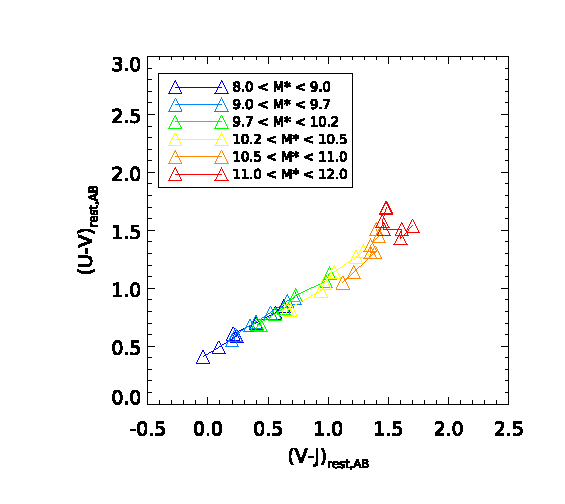
\includegraphics[width=0.5\textwidth]{uvj_track} &
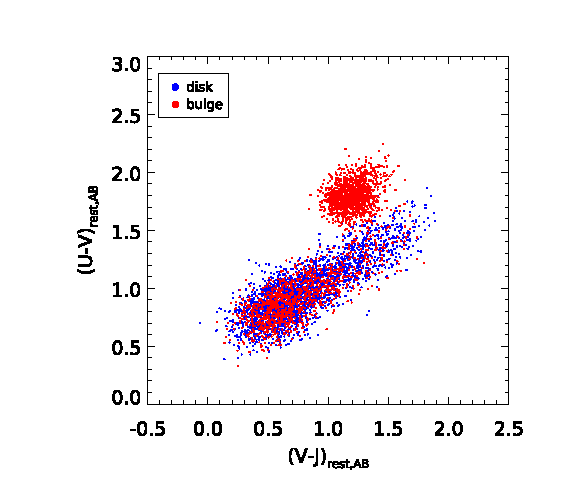
\includegraphics[width=0.5\textwidth]{uvj_gen}
\end{tabular}
\caption{\label{FIG:uvj_track} {\bf Left:} Observed median colors of galaxies of different masses, for different redshift (from $z=0.3$ to $z=3.0$). The trend is that galaxies move diagonally toward the bottom-left corner when going to higher redshifts. {\bf Right:} Generated \uvj colors of disk (blue) and bulge (red) components of galaxies with $\mstar > 10^9\,\msun$ and $0.8 < z < 1.2$.}
\end{figure}

This parametrization will generate a \uvj diagram very similar to the observed one, with the same redshift and mass trends. However, the observed \uvj diagram is made out of the \emph{total} light of the galaxy. Here we need to decompose the galaxy into a bulge and a disk component, and both have usually different colors. The way I chose to handle this is to always use the ``active'' \uvj colors for disk components, always use the ``passive'' \uvj colors for bulges of bulge-dominated galaxies ($B/T>0.6$), and randomly use either the ``passive'' or the ``active'' \uvj colors for the bulges of intermediate galaxies ($B/T<0.6$) with $50\%$ probability each.

The resulting \uvj colors are shown in \rfig{FIG:uvj_track} (right).


\subsection{Choosing an optical SED}

To go beyond the colors and associate a full optical SED to the galaxies (and their bulge/disk components), the idea is to consider that there is an average SED for each position on the \uvj diagram, and that one can attribute this average SED to the galaxies that are at this position.

Therefore I have binned the \uvj plane into small buckets of about $0.1$ mag, and computed the observed average rest-frame SED of all the galaxies that fall inside each bucket. I also split the sample in redshift bins, to further refine the SEDs, but this turned out to have negligible impact. These rest-frame SEDs are actually generated by FAST, which is the code that Maurilio Pannella used to estimate stellar masses in the first place, and are created from the Bruzual \& Charlot (2003) stellar population models. These SEDs are output by FAST in observed-frame, so I first de-redshift them, normalize them by the total stellar mass of the galaxy, interpolate them on a common rest-frame wavelength grid, and compute the average for each wavelength. The result is a wide library of about $850$ reference SEDs, all normalized per unit stellar mass.

Then the procedure is simply to pick one of these SEDs depending on the position of the galaxy in the \uvj diagram. If the average SED is made out of less than $10$ observed galaxies, the bin is considered as unreliable and the average SED of the closest reliable bin on the \uvj plane is chosen instead.

I run this procedure for both disk and bulge components, multiply the chosen SEDs by the respective stellar mass of each component, redshift them to the redshift of the galaxy, and finally integrate the resulting SED over the chosen UV-NIR passbands.


\subsection{Choosing an IR SED}

The generation of the IR fluxes is the same as the one we used before, either for my paper, or to generate the \herschel images with the previous Astrodeep mock catalog. Basically, we use the Chary \& Elbaz (2001) library of FIR SEDs, normalize them to unit $\lir$, and attribute one of these SEDs to every galaxy, from its redshift and ``starburtiness'' (see \rsec{SEC:sfr}). At higher redshifts, galaxies have warmer dust temperatures (Magdis et al.~2012), and the dust temperature also correlates with the offset of a galaxy from the Main Sequence (Magnelli et al.~2014). We use here the redshift evolution that was seen when I stacked \herschel images for my paper, and the starburstiness trend is put by hand (I'm not sure it has an important effect though).

Then, as for the optical flux computation, the chosen SED is multiplied by the $\lir$ of the galaxy, redshifted, and integrated over the chosen IR passbands to produce the final flux. Note that I chose to attribute all of the FIR flux to the ``disk'' component. This should not matter, since at these wavelengths we usually do not have the resolution to disentangle between bulge and disk.

Lastly, to properly reproduce the SPIRE fluxes ($250$, $350$ and $500\,\um$), I had to boost them up by $30\%$. This may be an issue of the SED library.


\subsection{Generating sky positions}

The final step is to generate a position on the sky for each galaxy. The procedure I used here is the same as the one I described earlier. To start with, I make very simplistic assumptions. First, I consider that the angular clustering does not evolve with redshift. This is probably wrong, since we know that galaxies are more clustered today than in the past. On the other hand, I work here in \emph{angular} correlation, not proper distance (say, in kpc). I assume the same angular correlation at $z=1$ and $z=0.5$ (e.g.), which means that galaxies will be clustered on the same angular scale. This angular scale will correspond to a smaller proper distance at $z=0.5$ than at $z=1$, so it will somehow mimic the increase of proper distance clustering with time. I don't know how far that is from the real observed trends though. Second, I consider that there is no sub-population of galaxies that are more clustered than the rest. E.g., massive early-type galaxies are treated the same way as, say, dwarf star-forming galaxies. This is probably wrong. For the FIR images however I did not care much, because both these populations will not contribute at all to the FIR flux, and we are mostly dominated by star-forming galaxies close to $\mstar = 3\times10^{10}$ -- $10^{11}\,\msun$ at all redshifts.

With that in mind, I first take the observed GOODS--South catalog from CANDELS, select all galaxies between $z=0.9$ and $z=1.1$ ($z_{\rm phot}$) and $\mstar > 10^9\,\msun$. I compute the two-point correlation function of this sample using the Landy-Szalay estimator (thanks to Catherine White!). I know that this correlation function is not ``pure'', in the sense that 1) the redshift range considered ($0.9 < z < 1.1$) is large ($\sim1\,{\rm Gpc}$); and 2) even if it weren't, our photometric redshifts are uncertain. There is not much I can do about point 1), since we have limited volume in CANDELS, and I need large statistics to build robust correlation functions. For point 2) however, the redshift uncertainties can be simulated, and I have done so.

My objective is then to simulate a similar correlation function from scratch. To do so, I first take a redshift slice of the mock catalog. I generate clustered positions using the Soneira \& Peebles algorithm (again, thanks to Catherine White!), with a fixed set of parameters (power law index equal to $0.4$, number of levels $N_{\rm level} = 4$, and I generate twice more sources than needed, then pick at random the ones I need among these). These parameters were fine tuned to reproduce the observed correlation functions (see below). It turns out that, doing so, one gets the right two-point correlation slope, but not the right amplitude: the correlation is too strong at all scale. To fix this, one has to say that there is a fraction ($60\%$) of the sample which is not clustered, and has uniformly random sky positions.

To make sure that these parameters are matching the ``real'' correlation function, I simulated redshift uncertainties to try to mimic the measurement that I did in GOODS--South. I took the ``true'' redshifts from the mock catalog, and added a Gaussian error proportional to $1+z$, with an error of $2\%$. I also added $20\%$ of ``outliers'' with $7\%$ relative error. These numbers were chosen to reproduce the distribution of redshift differences found when comparing our CANDELS redshifts against the 3DSHT redshifts. Re-slicing the catalog with these ``uncertain'' redshifts and computing the correlation function, one recovers exactly the observed correlation.

Also, as a double check, I computed the angular correlation function of the whole catalog above $\mstar > 10^{10}\,\msun$, mixing all redshifts all together. This way, I get rid of the issue of the redshift uncertainty, and the agreement is also very good. I have also tried to look at different sub-samples, like \herschel detections only, massive star-forming galaxies, massive passive galaxies, and it turned out that the correlation function was more or less always the same.


\section{Results}

I will use two diagnostics to assess the quality of this mock catalog. The first one is the flux distribution of the whole catalog, and the second is the pixel distribution of simulated images (for confused FIR images where blending is important).

In what follows, I use a mock catalog generated with $90\%$ completeness in $H$-band down to $H=29$, from $z=0.01$ to $z=6$. Over $17\times17\,{\rm arcmin}$, this represents $104\,000$ galaxies. The minimum stellar mass goes as low as $5\times10^4\,\msun$ at $z=0.01$, and rises with redshift to reach $7\times10^6\,\msun$ at $z=1$, and $10^8\,\msun$ at $z=4$.


\subsection{Optical magnitudes}

\begin{figure}
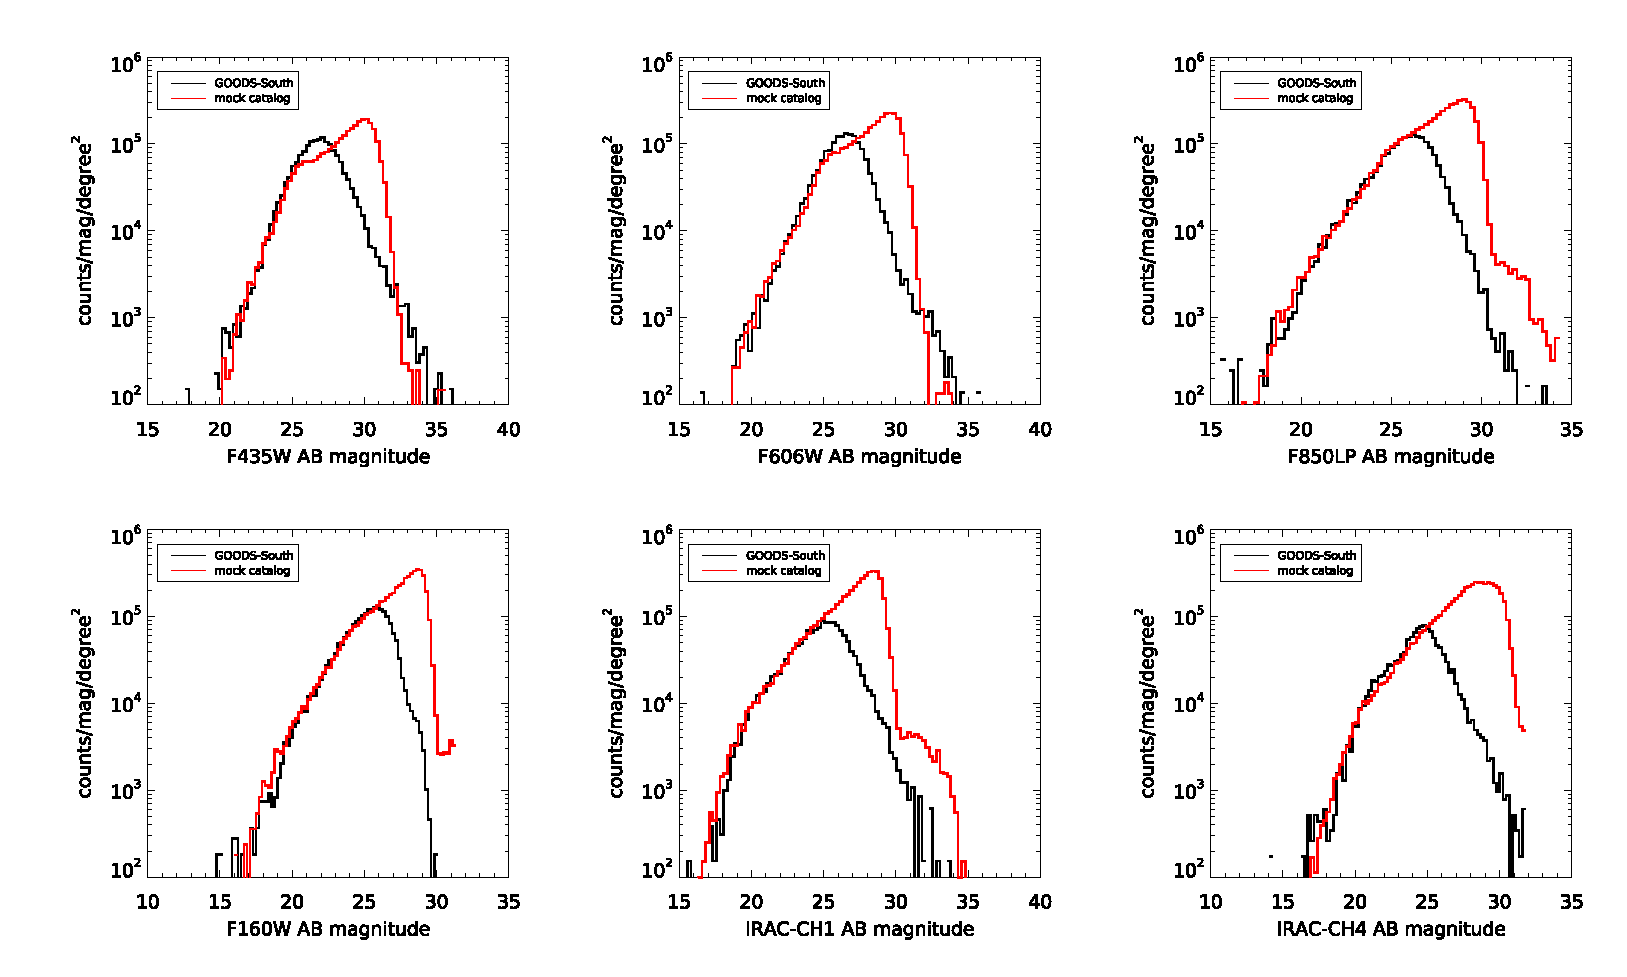
\includegraphics[width=\textwidth]{mags}
\caption{\label{FIG:mags} Total magnitude distribution of the real GOODS--South catalog (black) and the mock catalog (red), in different \hst bands and \spitzer IRAC.}
\end{figure}

\rfig{FIG:mags} is showing the agreement of the total magnitude distribution, in multiple bands. This agreement is very good in the NIR. Since these wavelengths are most closely correlated to the stellar mass of the galaxies, and since the mock catalog was built to reproduce exactly the stellar mass function in GOODS--South, this should not come as a surprise. Still, this shows that the procedure works well. The situation in the UV-optical (F435W and F606W) is not perfect though, as you can see there is a bending at faint magnitudes close to $25$ magnitude. I'm not sure where this comes from though, but it seems to originate from low-redshift low-mass galaxies, which are probably not blue enough in the mock catalog. Maybe that could be fixed by tweaking the redshift splitting of the SED library.


\subsection{FIR fluxes}

\begin{figure}
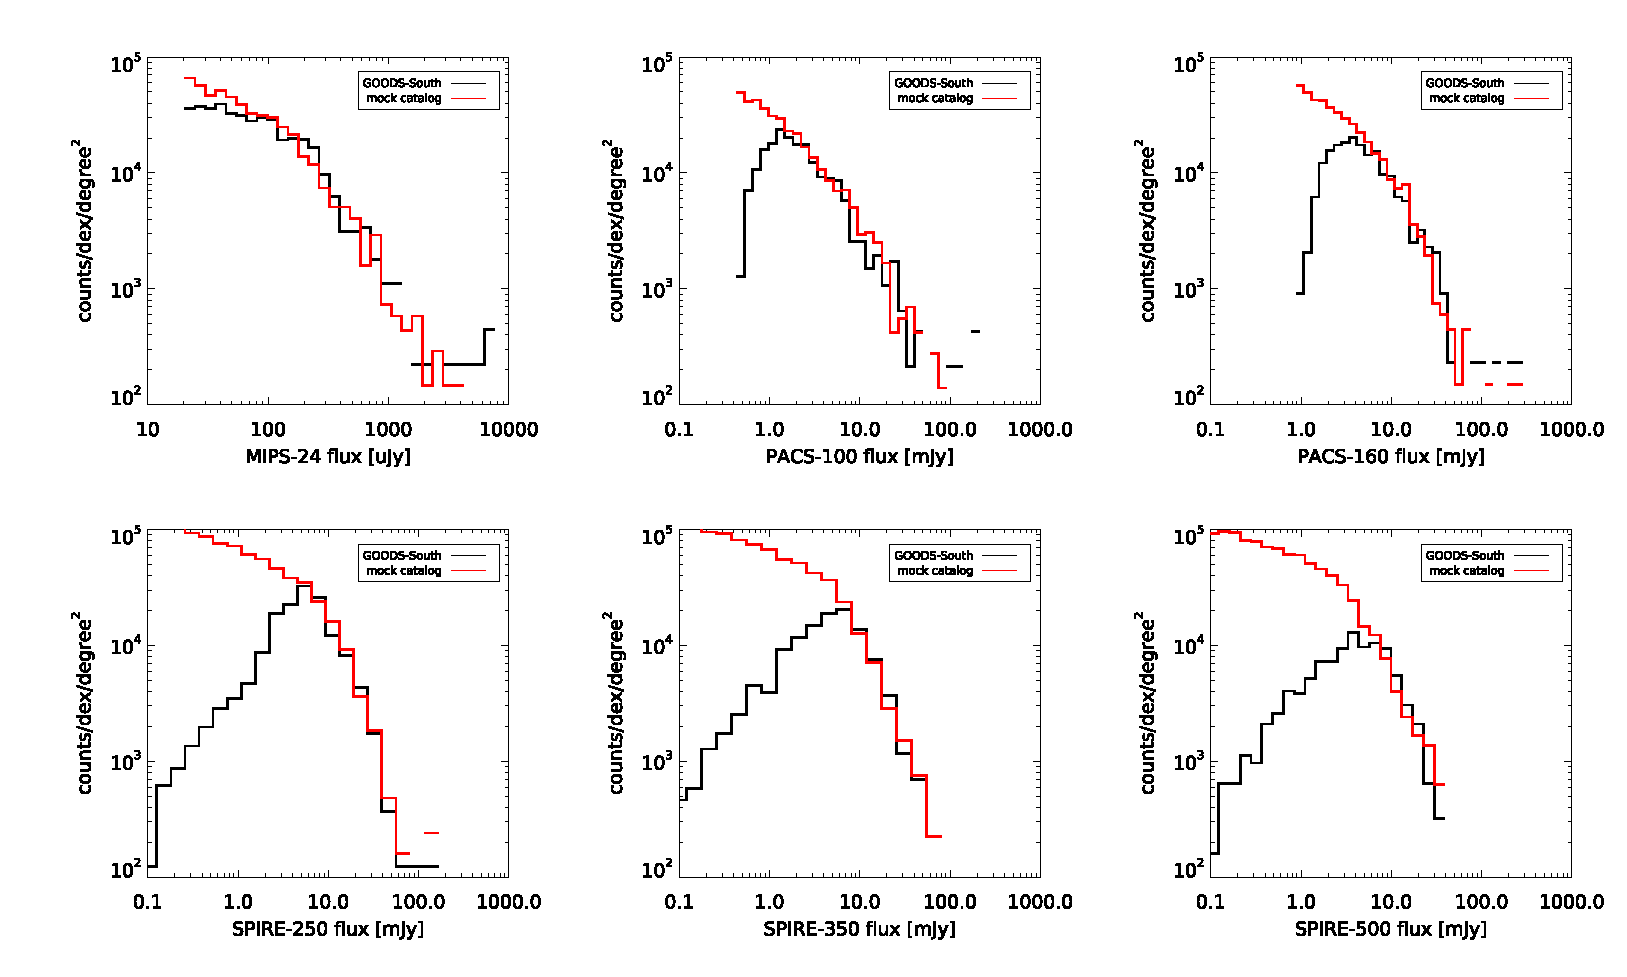
\includegraphics[width=\textwidth]{ir_flux}
\caption{\label{FIG:irflux} Total flux distribution in the MIR to FIR of the real GOODS--South catalog (black) and the mock catalog (red).}
\end{figure}
\begin{figure}
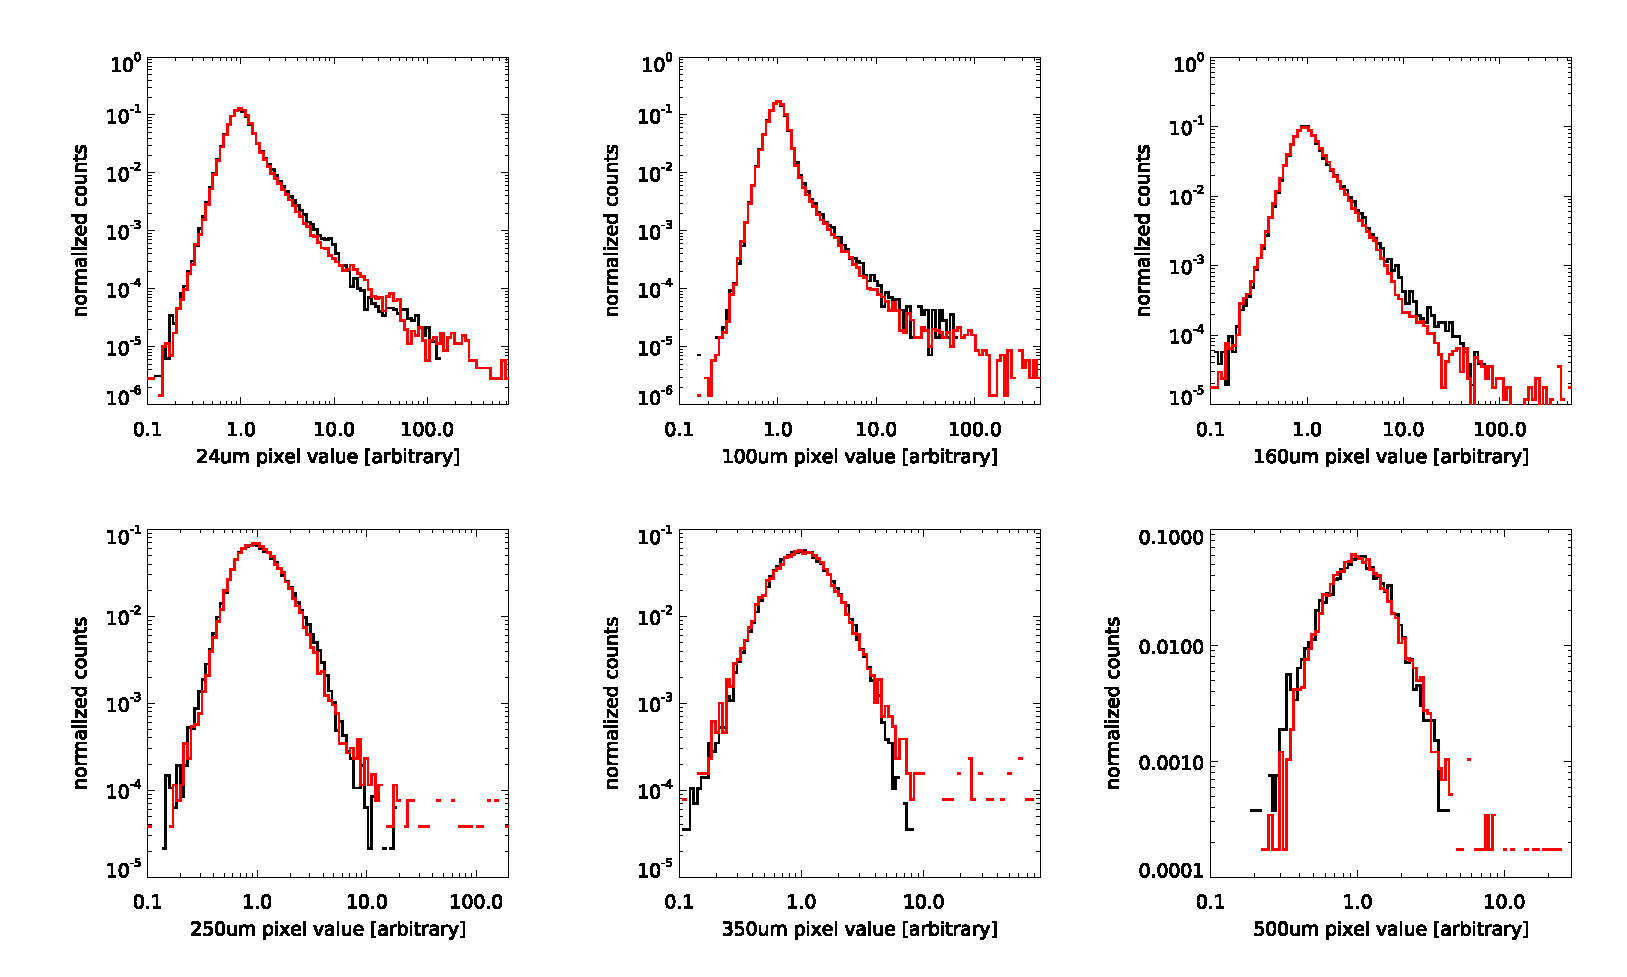
\includegraphics[width=\textwidth]{ir_pd}
\caption{\label{FIG:irpd} Pixel histogram distribution of the simulated FIR images versus real images in GOODS--South.}
\end{figure}

\rfig{FIG:irflux} shows basically the same plots, but with the FIR fluxes. Here the agreement is very good, there is really nothing to say. Same goes for \rfig{FIG:irpd}, where I compare the pixel histogram distribution of the simulated maps against the observed maps. This second test is important because of the blending, which sometimes pollutes the measured flux catalogs (two sources are combined into a single one), which tends to produce more bright fluxes than there actually is in the real Universe. By analyzing the map statistics directly, one gets rid of this issue of the counter part identification.


\end{document}

